\chapter{Алгоритмы}

\begin{multicols}{2}
    \raggedcolumns

    \section{Анализ алгоритмов. Понятие о сложности по времени и по памяти. Асимптотика, О-
    символика. Доказательство корректности алгоритмов.}
    \begin{definition}{(O-нотация)}{}
        Пусть $f,g: \ \N \to \N$. Тогда $f = \bigOO(g)$, если $\exists C > 0$ и $\exists N: \ \forall n > N$:
        \[
            f(x) \leq Cg(x)  
        \]
    \end{definition}
    \begin{proposition}{}{}
        $f = \bigOO(g) \Leftrightarrow \exists C > 0 \ \forall n \in \N: \ f(n) \leq Cg(n).$
    \end{proposition}
    \begin{definition}{}{}
        $f, g: \ \N \to\N$. Тогда $f = \Omega(g)$ или $g = \bigOO(f)$ или $\exists C > 0\ f(n) \geq Cg(n).$
    \end{definition}
    \begin{definition}{}{}
        $f = \Theta (g)$, если $f = \bigOO(g)$ и $g = \bigOO(f)$ или $\exists C_1, C_2 > 0\ \forall n \in \N C_1 g(n) \leq f(n) \leq C_2g(n)$.
    \end{definition}
     Примеры:
     \begin{multicols}{2}
        \begin{itemize}
            \item $n = \bigOO(n^2), \ \mathmbox{n^2 = \Omega(n);}$
            \item $n\log n = \bigOO(n^2)$;
            \item $3n + n^2 = \Theta(n^2)$;
            \item $\log^{10} n = \bigOO(n^{1/5}).$
        \end{itemize}
     \end{multicols}
     \begin{theorema}{(Мастер Теорема)}{}
        Пусть $T(n)$ -- время работы какого-то алгоритма на входе длины $n$, причем $T(n) = aT(\dfrac{n}{b}) + f(n)$. Тогда 
        \begin{enumerate*}
            \item Если $\exists \varepsilon > 0: \ f(n) = \bigOO(n^{\log_ba - \varepsilon})$, то \[
                T(n) = \Theta(n^{log_ba})  
            \]
            \item Если $f(n) = \Theta (n^{\log_ba})$, то 
            \[
                T(n) = \Theta (n^{log_ba}\cdot \log n)
            \]
            \item Если $\exists \varepsilon > 0: \ f(n) = \Omega(n^{\log_ba + \varepsilon})$, причем $\exists c<1: \ \mathmbox{a\cdot f^{n/b} \leq c\cdot f(n)}$, ($\forall n$, начиная с некоторого), то $T(n) = \Theta (f(n))$.
        \end{enumerate*}
     \end{theorema}
     \cons Пусть $T(n) = 2T(n/2) + \Theta(n)$. Тогда $T(n) = \Theta(n\log n)$.
     \par
     \myexe{Префиксные суммы.} Пусть $a_1, \ldots, a_n$ -- статический массив. $l,r$ -- индексы. Сообщить $a_l + a_{l+1} + \ldots + a_r$
     \par
     \begin{itemize}
        \item[] Наивное решение: $\bigOO(n\cdot q)$, где $q$ -- количество запросов;
        \item[] Префиксные суммы:
        \begin{algorithmic}[1]
            \State pref[$0$] = $0$
            \State pref[$i$] = $a_1 + \ldots + a_i$
            \State pref[$i+1$] = $a_1 + \ldots + a_i + a_{i+1}$
        \end{algorithmic}
        Это проходит за $\bigOO(n)$. Итого
        \[
            a_l + \ldots a_r = pref[r] - pref[l-1]  
        \]
        Решение $\bigOO(n+q)$
     \end{itemize}
     \myexe{Бинарный поиск} Отсортированный массив $a_1 \leq a_2 \leq \ldots \leq a_n$. Вопрос: есть ли $x$ в этом массиве.
     \begin{itemize}
        \item[] Наивное: $\bigOO(n\cdot q)$
        \item[] $\bigOO(q\cdot \log n + n)$
        Пусть $l=1, \ r=n$. $x$ лежит в отрезке $[l,r]$. Посмотрим на середину массива с индексом $m = \dfrac{l+r}{2}$. Тогда:
        \begin{enumerate*}
            \item Если $a[m]=x$ -- выдать да;
            \item Если $a[m] < x$, то ответ справа $l=m$, повторяем;
            \item Иначе $r=m$.
        \end{enumerate*}
        \begin{algorithmic}[1]
            \Repeat 
            \State int $m = \dfrac{(l+r)}{2}$
            \If  $a[m] == x$
            \State Выдать $yes$
            \ElsIf $a[m]<x$
            \State $l = m$
            \Else 
            \State $r=m$ 
            \EndIf
            \Until $(r-l>1)$
            \If ($a[l] == x || a[r] == x$)
            \State Выдать $yes$
            \Else
            \State Выдать $no$
            \EndIf
        \end{algorithmic}
     \end{itemize}
    \section{Строки и операции над ними. Представление строк. Вычисление длины, конкатенация.
    Алгоритмы поиска подстроки в строке.}

    \section{Сортировки. Нижняя теоретико-информационная оценка сложности задачи сортировки.
    Алгоритмы сортировки вставками, пузырьком, быстрая сортировка, сортировка
    слиянием. Оценка сложности.}
    \subsection*{Сортировки}
    Постановка задачи: Дан массив объектов $a_1,\ldots, a_n$. На объектах задано отношение порядка:
    \[
        \forall x,y, \hspace*{0.5cm} x < y \text{ или } x = y \text{ или } x > y
    \]  
    Цель: переставить элементы, чтобы они шли в порядке неубывания (невозрастания). Или также найти перестановку: $\sigma:\ [n] \to [n]$:
    \[
        a_{\sigma(1)} \leq a_{\sigma(2)} \leq \ldots \leq a_{\sigma(n)}  
    \]
    \begin{theorema}{}{}
        Любой алгоритм сортировки, основанный на сравнениях, требует $\Omega(n\log n)$ сравнений в худшем случае на массиве длины $n$. 
    \end{theorema}
    \begin{lemma}{}{}
        $\log (n!) = \Theta(n\log n)$
    \end{lemma}
    \subsubsection*{Сортировка слиянием}
    Сортировка за $\bigOO(n\log n)$, основанная на сравнениях.
    Разобьем массив на два равных куска:
    \begin{center}
        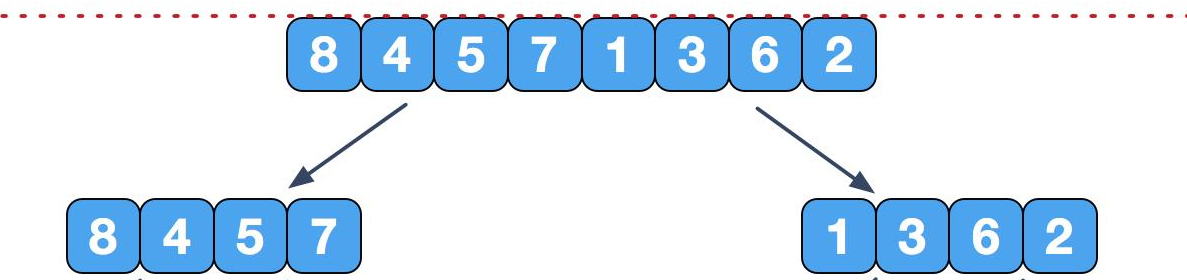
\includegraphics[scale=0.25]{images/1st_step.png}        
    \end{center}
    Рекурсивно продолжаем:
    \begin{center}
        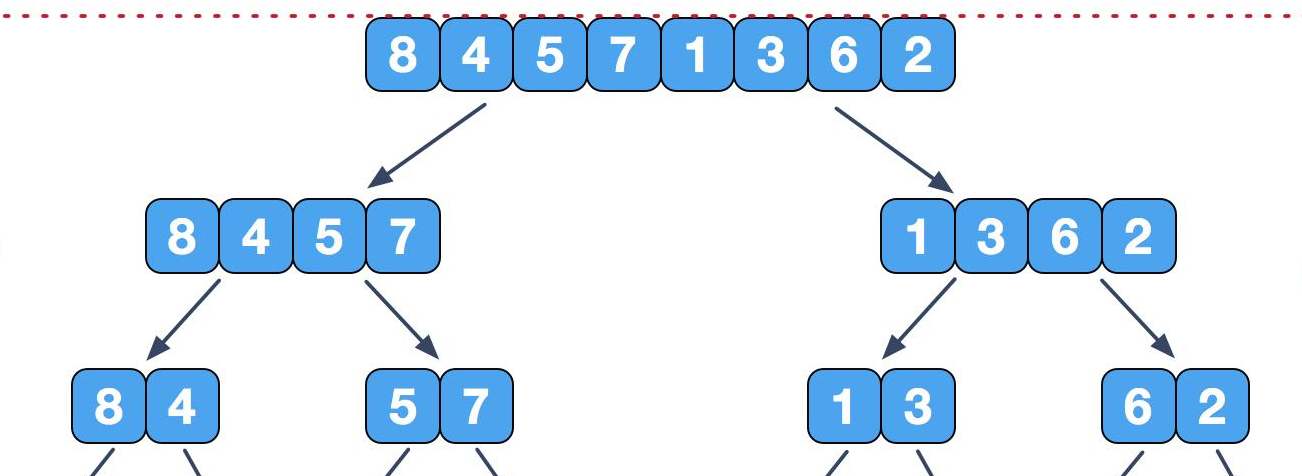
\includegraphics[scale=0.25]{images/2nd_step.png}
    \end{center}
    Следующий шаг:
    \begin{center}
        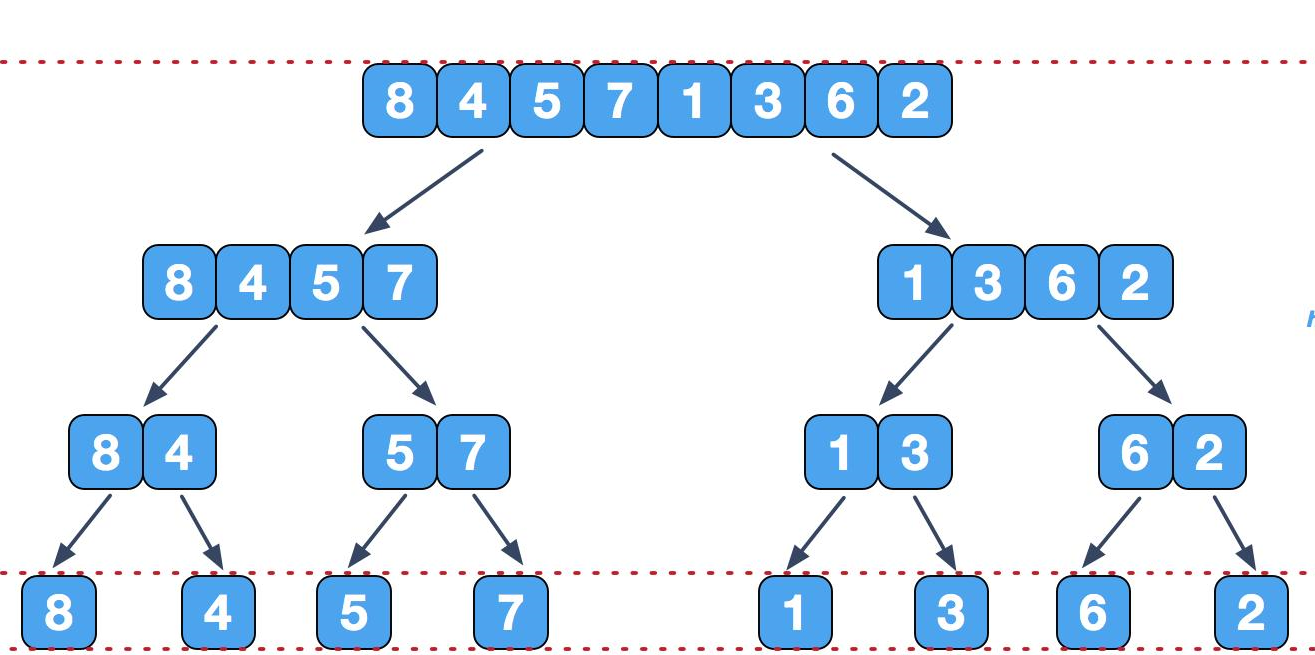
\includegraphics[scale=0.25]{images/3rd_step.png}
    \end{center}
    Сортируем полученное:
    \begin{center}
        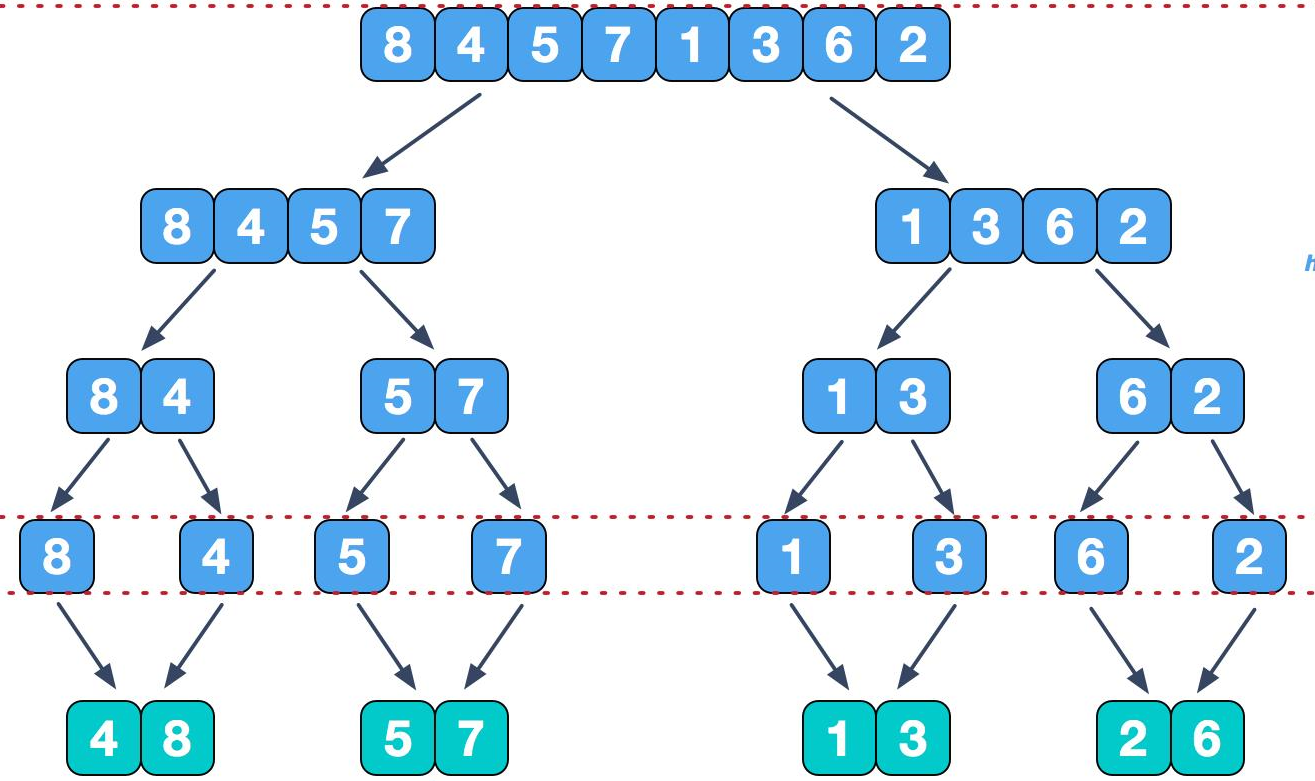
\includegraphics[scale=0.25]{images/4th_step.png}
    \end{center}
    Склеиваем:
    \begin{center}
        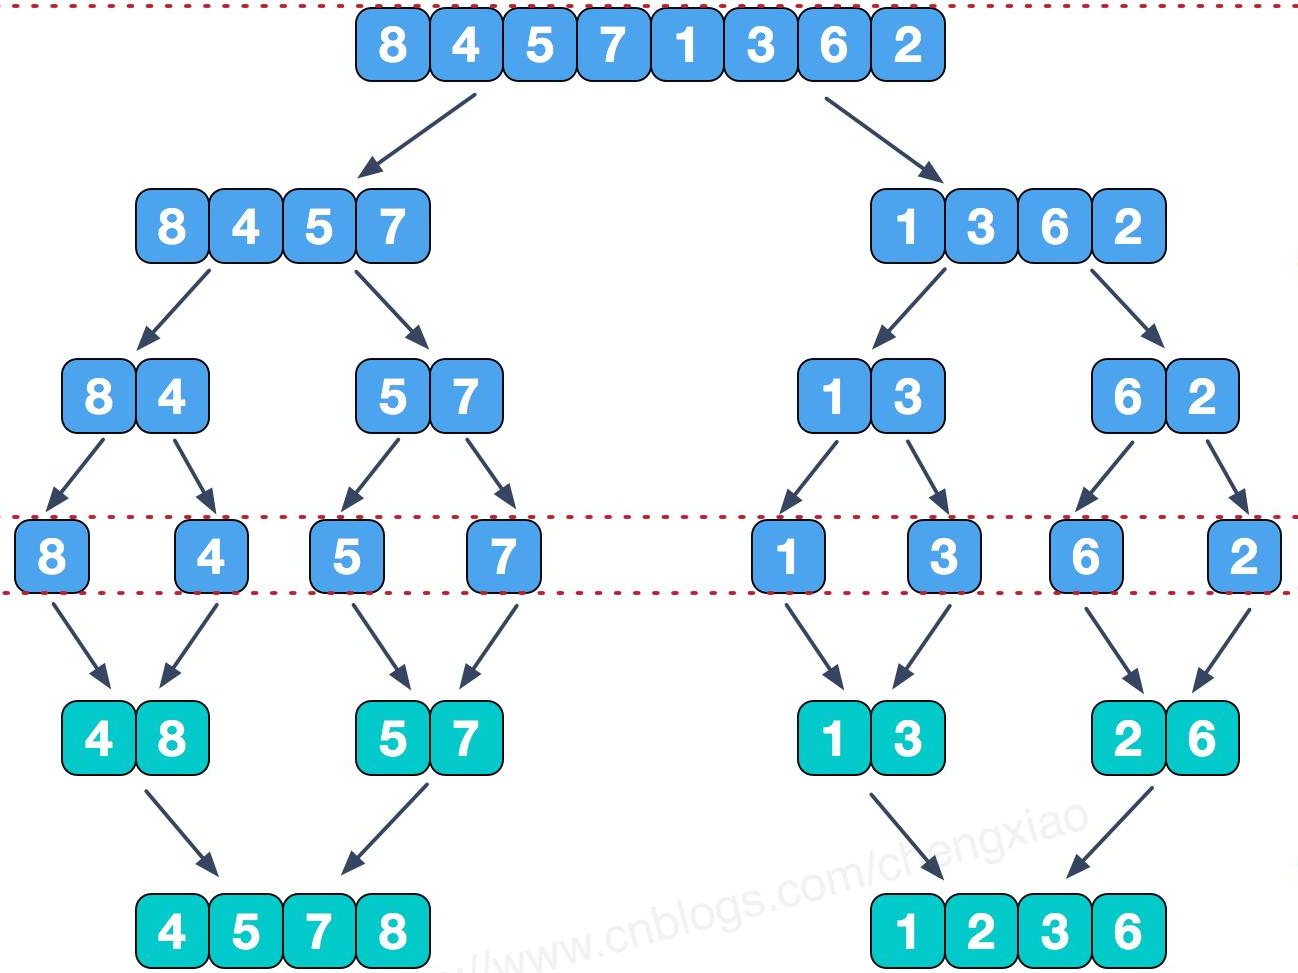
\includegraphics[scale=0.25]{images/5th_step.png}
    \end{center}
    Заводим два указателя на отсортированные части. Записываем минимальное из элементов указателя и сдвигаем тот, который записали, повторяем:
    \begin{center}
        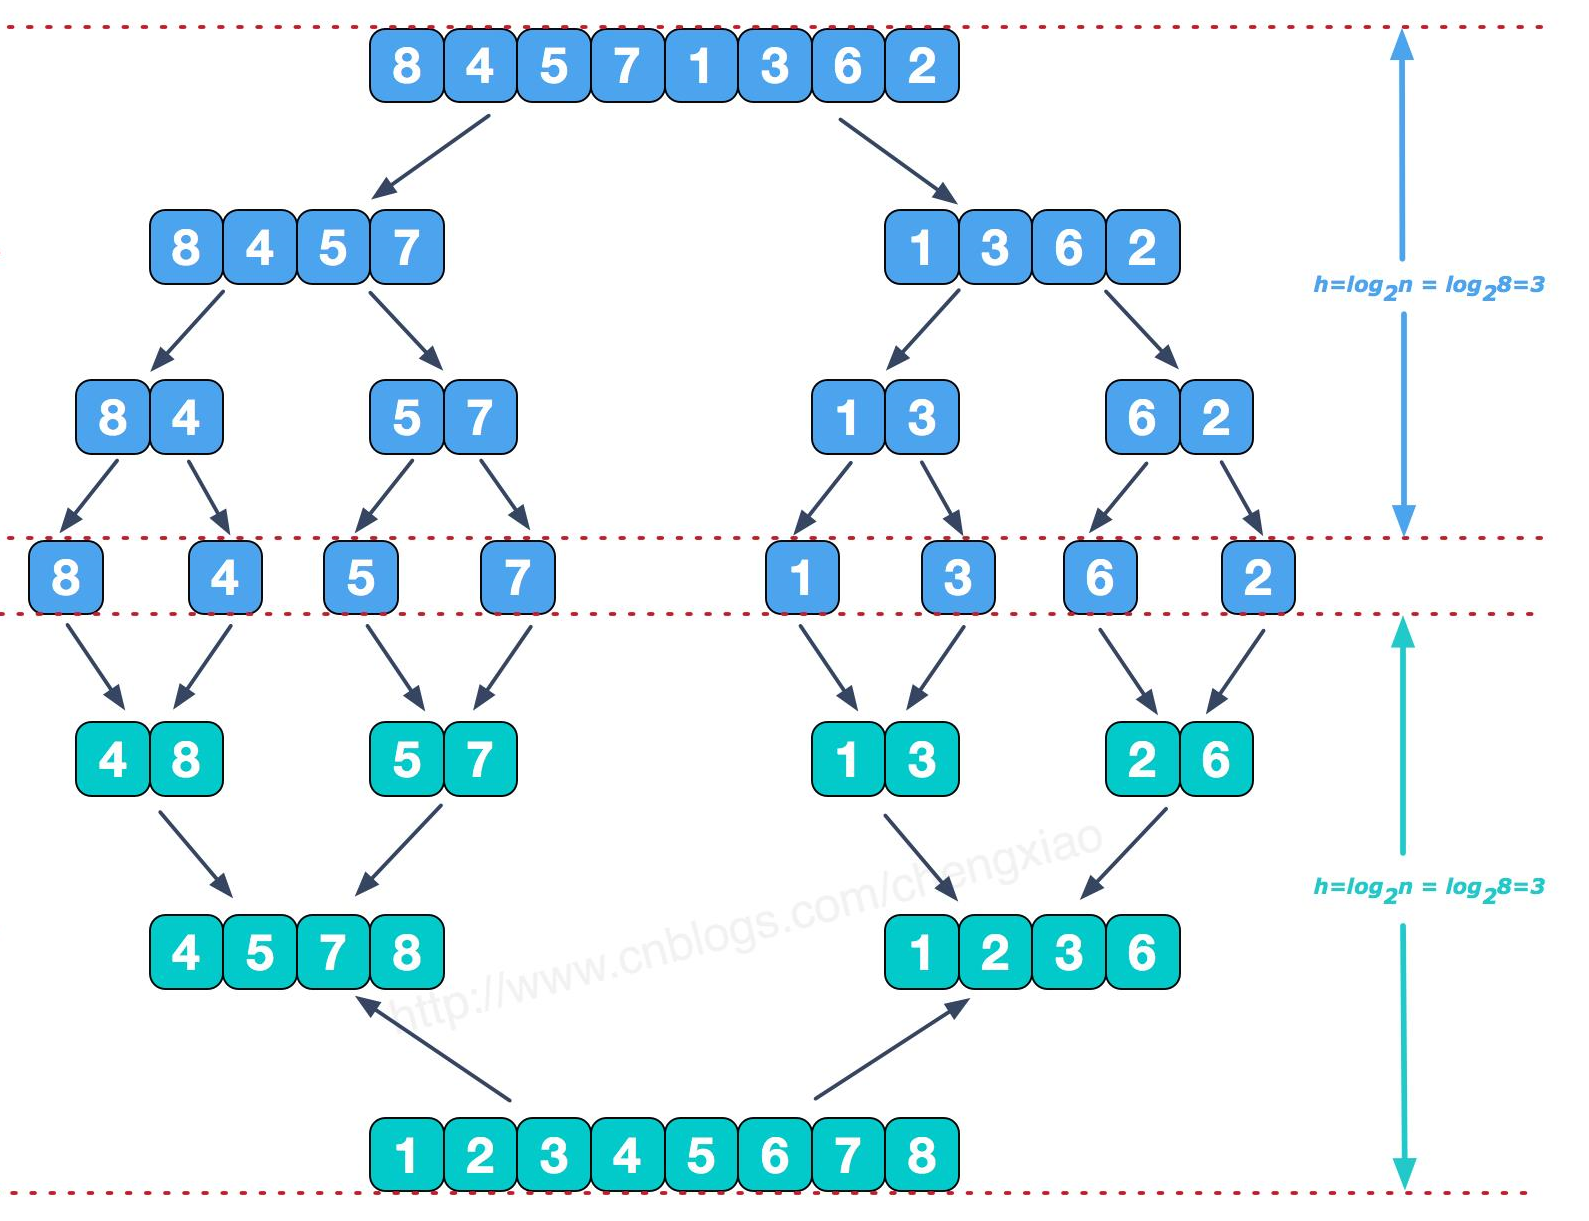
\includegraphics[scale=0.2]{images/Full.png}
    \end{center}
    Псевдокод:
    \begin{algorithmic}[1]
        \Function{MergeSort}{A}
        \If len(A) == 1 
        \State \Return
        \EndIf
        \State B, C -- две половины A
        \State MergeSort(B)
        \State MergeSort(C)
        \State Merge(B,C,A)
        \EndFunction
        \Function{Merge}{B,C,A}
        \State i=0, j=0, p=0
        \Repeat  
        \If (B[i] < C[j])
        \State A[p++] = B[i]
        \State ++i
        \Else
        \State A[p++] = C[j]
        \State ++j
        \EndIf
        \Until (i < len(B) and j < len(C))
        \Repeat 
        \State A[p++] = B[i]
        \State ++i
        \Until (i < len(B))
        \Repeat 
        \State A[p++] = C[j]
        \State ++j
        \Until (j < len(C))
        \EndFunction
    \end{algorithmic}
    \subsubsection*{Количество инверсий}
    Неотсортированный массив $a_1, \ldots, a_n$. Инверсия $(i, j): \ i < j, \ a_i > a_j$. Пусть $f(A)$ -- число инверсий в массиве $A$. $f(A) = f(B) + f(C) + $ количество инверсий, пересекающих разделитель. В момент, когда выбирается $B[i]$ все числа, стоящие слева от $B[i]$ его меньше, причем там ровно $j$ элементов из $C$. К ответу добавить $j$.
    \subsubsection*{Нерекурсивная реализация MergeSort}
    Будем считать, что $n$ -- степень двойки. (Если нет, то добавим слева или справа меньшие или большие, соответственно элементы, чем остальные в массиве. После сортировки их выкинем)
    \begin{algorithmic}[1]
        \Function{MergeSort}{a}
        \State queue<vector<int>> q
        \For{(int i = 0; i < n; ++i)}
        \State q.push({a[i]})
        \EndFor
        \While{(q.size() > 1)}
        \State vector<int> a = q.front()
        \State q.pop()
        \State vector<int> b = q.front()
        \State q.pop()
        \State q.push(Merge(a,b))
        \EndWhile
        \EndFunction
    \end{algorithmic}
    Ответ: $q.front()$. Время: $\bigOO(n\log n)$, Память: $\bigOO(n)$
    \subsection*{Быстрая сортировка (Quick sort)}
    Массив чисел: $a_1, \ldots, a_n$. Пусть $x$ -- случайный элемент массива. $Partition(A, x)$ -- перемешивание массива в виде: 
    \[
    \underbrace{[\hspace*{0.2cm} < x \hspace*{0.2cm}]}_{\substack{Quick\\Sort}}[\hspace*{0.2cm} = x \hspace*{0.2cm}] \underbrace{[\hspace*{0.2cm} > x \hspace*{0.2cm}]}_{\substack{Quick\\Sort}}
    \]
    Псевдокод
    \begin{algorithmic}[1]
        \Function{QuickSort}{A}
        \If (len(A) == 1)
        \State \Return
        \EndIf
        \State x -- случайный элемент $A$
        \State Partition(A,x)
        \State B -- числа <= x, C -- числа > x
        \State QuickSort(B)
        \State QuickSort(C)
        \EndFunction
    \end{algorithmic}
    В худшем случае: $\Omega(n^2)$.
    \begin{theorema}{}{}
        Математическим ожиданием времени работы на массиве длины $n$ есть $\Theta(n\log n)$.
    \end{theorema}
    \subsection*{Сортировка вставками (InsertSort)}
    Псевдокод 
    \begin{algorithmic}[1]
        \Function{InsertSort}{a}
        \If (len(A) == 1)
        \State \Return
        \EndIf
        \For{(i=1; i < n; ++i)}
        \State j = i-1
        \While{(j >= 0 and a[j] > a[j+1])}
        \State swap(a[j], a[j+1])
        \State --j
        \EndWhile
        \EndFor
        \EndFunction
    \end{algorithmic}
    Худший случай -- массив отсортирован в обратном порядке. Сложность $\bigOO(n^2)$
    \begin{center}
        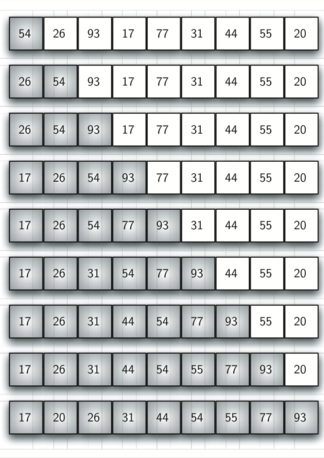
\includegraphics[scale=1.2]{images/insertsort.png}
    \end{center}
    \subsection*{Сортировка пузырьком (BubbleSort)}
    Псевдокод
    \begin{algorithmic}[1]
        \Function{BubbleSort}{a}
        \For{(int i = 0; i < n-2; ++i)}
        \For{(int j = 0; j < n-2; ++j)}
        \If a[j] > a[j+1]
        \State swap(a[j], a[j+1])
        \EndIf
        \EndFor
        \EndFor
        \EndFunction
    \end{algorithmic}
    Сложность: $\bigOO(n^2)$
    \subsubsection*{Оптимизация}
    \begin{enumerate*}
        \item После $i$ итераций, в конце $i$ чисел отсортировано;
        \begin{algorithmic}[1]
            \Function{BubbleSort}{a}
            \For{(int i = 0; i < n-2; ++i)}
            \For{(int j = 0; j < n-i-2; ++j)}
            \If a[j] > a[j+1]
            \State swap(a[j], a[j+1])
            \EndIf
            \EndFor
            \EndFor
            \EndFunction
        \end{algorithmic}
        \item Если не было $swap$, то массив уже отсортирован.
        \begin{algorithmic}[1]
            \Function{BubbleSort}{a}
            \State i=0
            \State isSwapped=True
            \While{isSwapped}
            \State isSwapped=False
            \For{(int j = 0; j < n-i-2; ++j)}
            \If a[j] > a[j+1]
            \State swap(a[j], a[j+1])
            \State isSwapped = True
            \EndIf
            \EndFor
            \State ++i
            \EndWhile
            \EndFunction
        \end{algorithmic}
    \end{enumerate*}

    \section{Представление матриц и векторов. Алгоритмы умножения матриц и эффективные
    способы их реализации. Численные методы решения систем линейных уравнений.}

    \section{Численное дифференцирование и интегрирование. Численные методы для решения
    систем дифференциальных уравнений.}

    \section{Граф. Ориентированный граф. Представления графа. Обход графа в глубину и в ширину.
    Топологическая сортировка. Подсчет числа путей в орграфе.}

    \section{Алгоритмы поиска кратчайших путей в графе. Алгоритм Дейкстры. Алгоритм Форда-
    Беллмана. Алгоритм Флойда. Алгоритм A*.}
    \columnbreak
    \section{Недетерминированные конечные автоматы, различные варианты определения.
    Детерминированные конечные автоматы. Их эквивалентность. Машина Тьюринга.}
\end{multicols}